\if0
衝撃試験の意味 要求
羽田先生の装置
図
印加方式

%質問事項 多かった
% 3軸印加について
% 公差等気にしすぎた

予備試験(日大、熊大)

自分でやったこと:字具作成(設計・加工) 
最初の加工:面取り、穴あけ、ねじきり
追加工(ねじ穴ミス)

本試験

キャリーケース損傷

全体スケジュール
当初と現実
\fi

%%%%%%%%%%%%%%%%%%%%%%%%%%%%%%%%%%%%%%

\section{衝撃試験(大野)}
 衝撃試験は,ロケットのフェアリング分離の際に衛星本体に衝撃が加わるために環境試験として行うことをJAXAから決められている.詳細は「衝撃試験ハンドブック」を参照.\\
 試験で求められていることは,
\begin{itemize}
 \item ATレベル+3dBの衝撃を,「3軸各方向に2回ずつ」加える
\end{itemize}
 ことによってハザード確認項目を満たし,衛星本体が壊れないことである.ATレベルに関しては「インターフェイス管理文書」,ハザード確認項目は「ハザードレポート」に記載されている.また,どちらについても「OP-S1-0013 EM衝撃試験計画書」にまとめてある.
 なお,本試験はEMについてのみ行う.

\subsection{使用装置}
 本試験で使用した装置を図\ref{fig4-4-1}に示す.衝撃試験の手法は多数あるが,私たちは熊本大学の波多先生が開発した「簡易式衝撃試験装置」を使用した.この装置は1回の打撃子の衝突により,XYZの全3軸同時に衝撃を印加することができる.\\
 詳細は「衝撃応答スペクトルにおける材料特性の影響評価」,第59回宇宙科学技術連合講演会講演集, No. P49, 2015. を参照.
\begin{figure}[H]
	\centering
	\includegraphics[scale=0.3]{04/fig/impact_device.jpg}
	\caption{熊本大の簡易式衝撃試験装置}
	\label{fig4-4-1}
\end{figure}
\subsection{準備(私がやったこと)}
この装置を用いて試験を行うにあたり,私が行ったことは
\begin{itemize}
 \item 試験計画書の作成
 \item ベース板の設計・加工
 \item 試験時の取りまとめ
 \item 報告書の作成
\end{itemize}
である.
\subsubsection{ベース板の設計・加工}
\begin{figure}[H]
	\centering
	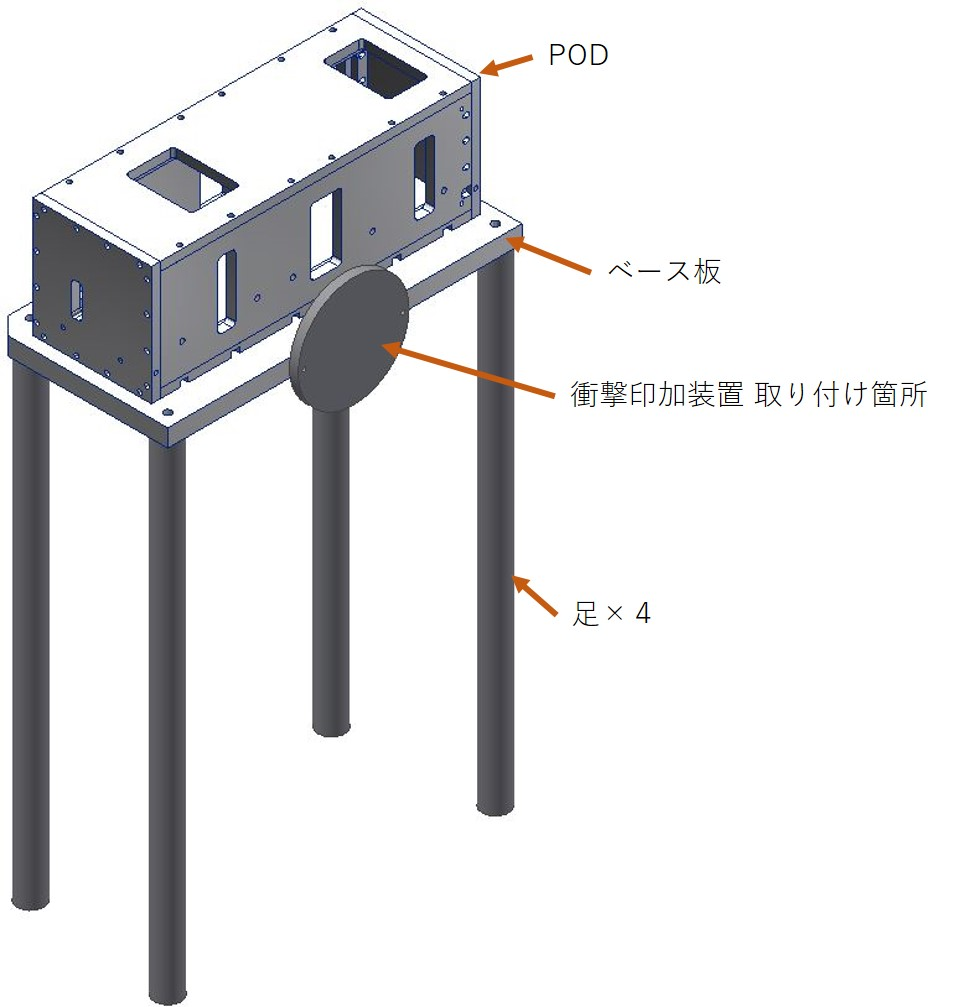
\includegraphics[scale=0.5]{04/fig/impact_base_board.jpg}
	\caption{衝撃試験で使用するベース板}
	\label{fig4-4-2}
\end{figure}
ベース板は,PODと接続される板であり,この板に衝撃印加装置と加速度計を取り付けて試験・測定を行う(図\ref{fig4-4-2}).測定物(今回では衛星)によってベース板のサイズ等が変わるため,自作する必要があった.必要な加工項目は
\begin{itemize}
 \item 板厚20mmの板を用意する
 \item 2箇所のC20の面取り(加速度計取り付け用)
 \item 足×4,加速度計×3,衝撃印加装置,PODをつけるための穴
\end{itemize}
であった.なお,当初の予定では面取りとPODの取り付け穴のみ加工をこちらで行い,他の加工はやっていただけることになっていたが,こちらの開発の遅れで波多先生側で時間が取れなくなり,全て加工することになった.\\
 加工自体はそれほど複雑ではなかった.また,構体系でも記載はあると思うが,工場の方が親身に手伝ってくれるので,不安があってもそれほど心配ない.ただし,人が多いときであると工場の方も手が回りきれないこともあるので,注意する必要がある.
また,加工は時間がかかるので,図面の作成を丁寧に行う(加工するときに寸法の計算をする必要のないように書く)ことと,前日までに加工順序をまとめておくことをお勧めする.\\
本加工でのミスは
\begin{itemize}
\item 発注時の面取りのし忘れ
\item 加速度計のねじ切りのピッチ
\end{itemize}
である.発注時の面取りは,ミスミであると無料でやってくれるのでやってもらう予定であった.これを忘れたことにより加工工程が増えてしまった.面取りは複雑な作業ではないが,面取りの大きさが大きかったので時間がかかった.
加速度計のねじきりのピッチは「細目」で指定されていたが,「並目」で加工してしまった.これにより,面取り部をさらに削るだけでなく,予備試験の際に気づいたので予備試験をもう1回やることになった.
些細なミスで開発の貴重な時間を失うので,当たり前ではあるが,必ずチェックしましょう.
\subsection{試験}
当初の予定では,
\begin{enumerate}
	\item ベース板の面取り加工を行う
	\item ベース板を熊大へ発送,追加工と衝撃印加方法の選定を行ってもらう
	\item 東工大にてEM衝撃試験を実施
\end{enumerate}
という流れであったが,開発の遅れと,加工のミスにより,下記行程に変更した.
\subsubsection{予備試験@日大}
\begin{figure}[H]
	\centering
	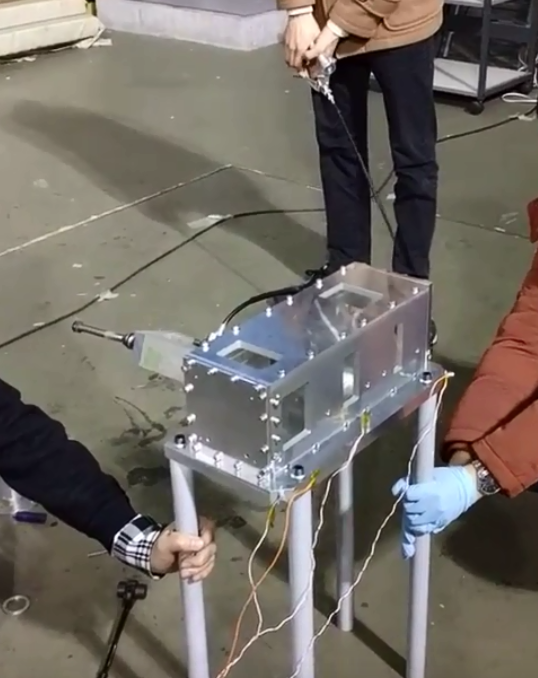
\includegraphics[scale=0.5]{04/fig/report_test_impact@nihon_univ.png}
	\caption{衝撃試験@日大}
	\label{fig4-4-3}
\end{figure}
開発の遅れから,熊大での加工・試験をあきらめ,日大で行われる衝撃試験に行き,日大の試験終了後に事前試験をやらせてもらうことになった(図\ref{4-4-3}).事前試験は池谷,山崎が参加した.前述にあったとおり,加速度センサの取り付けねじのピッチに誤りがあったため,再度実施することとなった.
\subsubsection{予備試験@熊大}
日大での予備試験での不具合から,ベース板を追加工し,熊本大にベース板を送り,再度衝撃印加方法の選定を行ってもらった.無事試験ができることになった.
\subsubsection{本試験@東工大}
当日はほとんどを波多先生にやっていただいたので,問題は特になかった.
\subsection{キャリーケースの損傷}
衝撃試験装置を東工大まで持ってきていただいたが,装置を入れていたキャリーケースが輸送中に破損してしまった.大きさによって最大重量が会社ごと決まっているので環境試験で荷物をつめる際には気をつけて欲しい.
\subsection{付録:全体スケジュール}
\begin{figure}[H]
	\centering
	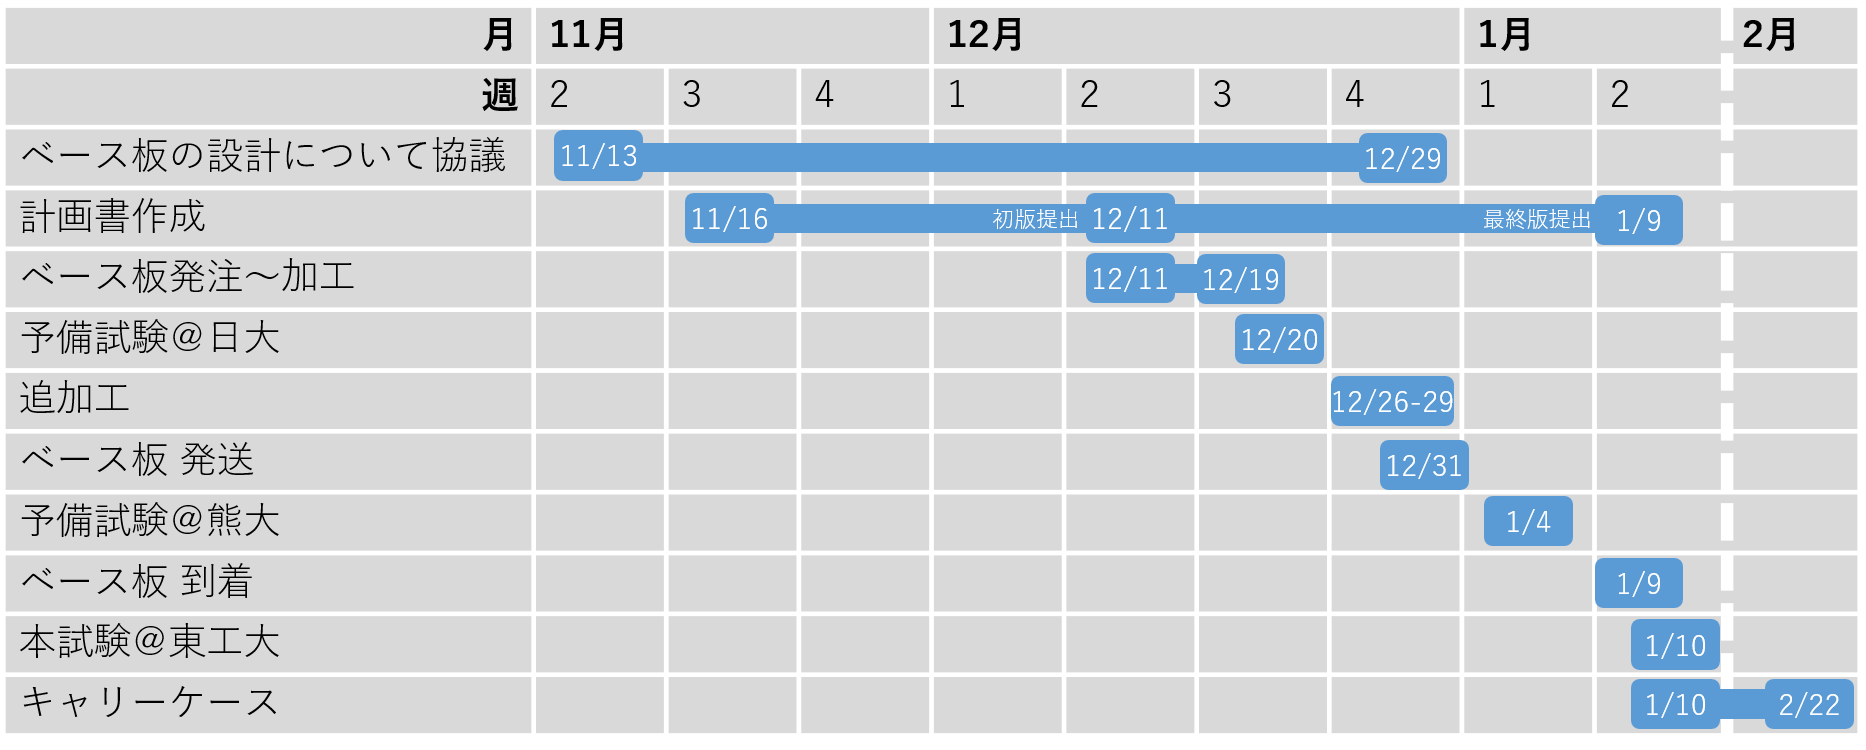
\includegraphics[scale=0.4]{04/fig/report_test_impact.png}
	\caption{衝撃試験スケジュール}
	\label{fig4-4-4}
\end{figure}
最後に本試験までのスケジュールを図\ref{fig4-4-4}に示す.これは,波多先生とのメールのやり取りから日付をまとめたものである.この日程でマージンはないのでこの日程で行うことはお勧めしない.余裕を持って開発を進めてもらいたい.






